% The sub section about the simulations technical data model
% @author Kalvin Döge
%

\subsection{Fachliches Datenmodel des Systems}\label{subsec:data-model}

Das fachliche Datenmodell für die Simulation ist wie folgt:

\begin{figure}[h]
    \centering
    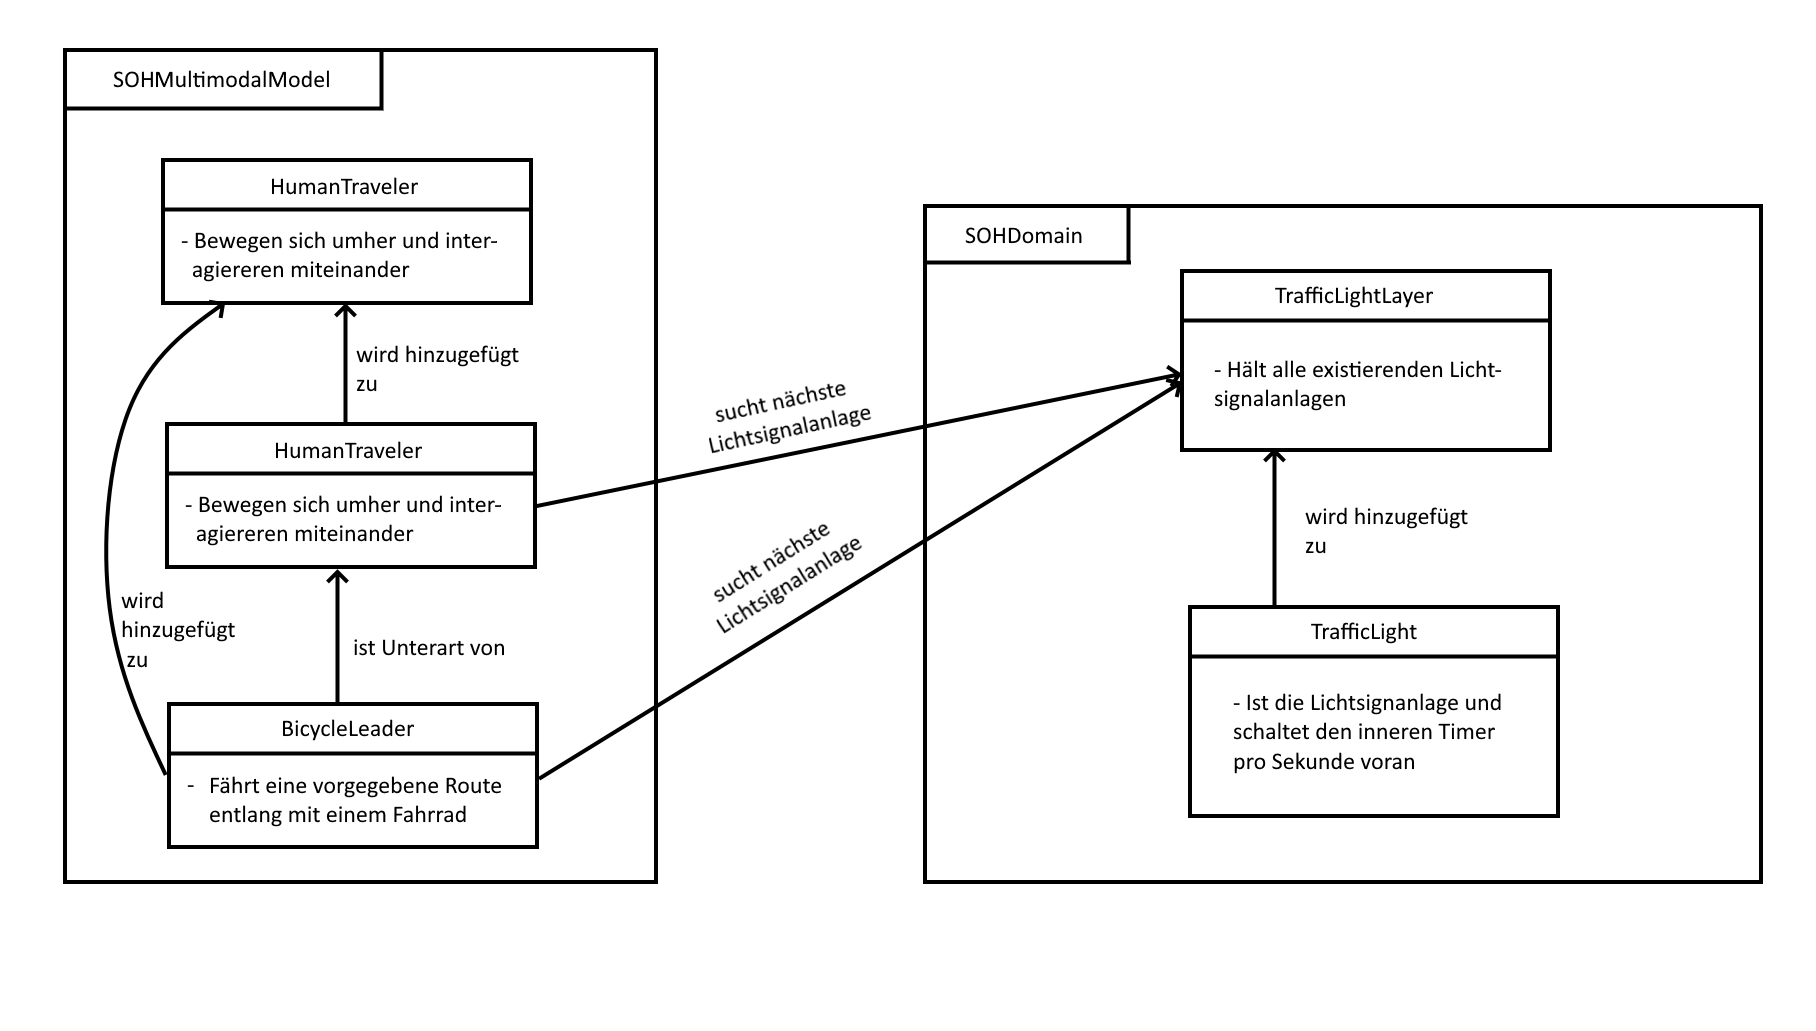
\includegraphics[width=0.75\textwidth]{architecture}
    \caption{Klassendiagramm der Agenten und Entitäten}
    \label{fig:class-diagramm}
\end{figure}

Zu der Grafik~\ref{fig:class-diagramm} sind folgende Erläuterungen wichtig, um das Zusammenspiel der einzelnen Elemente zu verstehen:

\textbf{HumanTraveler aus der SOHMultiModal-Komponente:}
\begin{itemize}
    \item Ist ein Agent in diesem System und kann Entscheidungen treffen zum Bewegen.
    \item \code{HumanTraveler}s können eine Modalität bei sich erschaffen, zum Beispiel ein \code{Bicycle}, \code{Car} oder zu Fuß gehen.
    Eines dieser Modalitäten ist dann ihr Transportmittel.
    \item Ein \code{HumanTraveler} besitzt die folgenden Eigenschaften:
    \begin{itemize}
        \item Eine Referenz auf ein Fahrrad, dem \code{Bicycle}, sollten sie eines besitzen
        \item Eine Referenz auf einen Pkw, dem \code{Car}, sollten sie eines besitzen
        \item Für alle verfügbaren Modalitäten noch eine Prozentangabe, die die Nutzungswahrscheinlichkeit der jeweiligen Modalität darstellt.
    \end{itemize}
    \item \code{HumanTraveler} haben dazu noch folgende Funktionen zum Nutzen:
    \begin{itemize}
        \item \code{Tick()} setzt den nächsten Agentenschritt fort, dass auch die Bewegung des \code{HumanTraveler}s beinhält und dem Agenten die Entscheidung zum Abbiegen gibt, sollte die Route das vorschlagen.
        \item \code{IsWaitingAtTrafficLight()} gibt einen Wahrheitswert zurück, ob der \code{HumanTraveler} aktuell an einer Lichtsignalschaltung wartet.
    \end{itemize}
\end{itemize}

\textbf{BicycleLeader aus der SOHMultiModal-Komponente:}
\begin{itemize}
    \item \code{BicycleLeader} sind identisch zu den \code{HumanTraveler}s, bis auf die Einschränkung, dass sie nur \code{Bicycle} nutzen beziehungsweise zu Fuß zum \code{Bicycle} gehen können.
    \item Ein \code{BicycleLeader} besitzt die folgenden Eigenschaften:
    \begin{itemize}
        \item Eine Referenz auf sein Fahrrad, dem \code{Bicycle}, sollte der BicycleLeader selbst eines besitzen und nicht ein gemietetes nehmen
    \end{itemize}
    \item \code{BicycleLeader} haben dazu noch folgende Funktionen zum Nutzen:
    \begin{itemize}
        \item \code{Tick()} setzt den nächsten Agentenschritt fort, dass auch die Bewegung des \code{BicycleLeader}s beinhält.
        \item \code{IsWaitingAtTrafficLight()} gibt einen Wahrheitswert zurück, ob der \code{BicycleLeader} aktuell an einer Lichtsignalschaltung wartet.
    \end{itemize}
\end{itemize}

\textbf{RouteFinder aus der SOHMultiModal-Komponente:}
\begin{itemize}
    \item \code{HumanTraveler} und \code{BicycleLeader} nutzen für das Erreichen ihres Zieles den \code{RouteFinder}, mit der sie eine Route zum Abfahren berechnet bekommen.
    \item Der \code{RouteFinder} hat die folgende Funktion und bietet sie nach außen an:
    \begin{itemize}
        \item \code{Search(Agent, Startpunkt, Zielpunkt, Modalitätenliste)} sucht für den Agenten von der Startposition zur Zielposition eine passende Route und beachtet dabei die Modalitäten, die der Agent nutzen kann.
    \end{itemize}
\end{itemize}

\textbf{HumanTravelerLayer aus der SOHMultiModal-Komponente:}
\begin{itemize}
    \item Der \code{HumanTravelerLayer} stellt die Umgebung für die \code{HumanTraveler} dar.
    \item \code{HumanTraveler} werden erschaffen und zu dem \code{HumanTravelerLayer} hinzugefügt.
    \item Die erschaffenen \code{HumanTraveler} bewegen sich auf dem \code{HumanTravelerLayer}, auf der sie mit anderen \code{HumanTraveler}s interagieren können.
    \item Zu jeder vollen Stunde wird ein \code{BicycleLeader} in dem \code{HumanTravelerLayer} hinzugefügt.
    \item Der erschaffene \code{BicycleLeader} bewegt sich ebenfalls auf dem \code{HumanTravelerLayer}.
    \item Der \code{HumanTravelerLayer} besitzt dabei folgende Eigenschaften:
    \begin{itemize}
        \item Die geographische Umwelt, die den digitalen Zwilling von Hamburg darstellt und alle Bewegungen festhält, als \code{SpatialGraphMediatorLayer}.
    \end{itemize}
\end{itemize}

\textbf{TrafficLight aus der SOHDomain-Komponente:}
\begin{itemize}
    \item \code{TrafficLight}s selbst sind Entitäten und sind statisch auf dem zugehörigen Layer.
    \item \code{TrafficLight}s können sowohl mit \code{HumanTraveler} als auch mit \code{BicycleLeader} in eine Warteschlange aufnehmen, sollte die aktuelle Lichtsignalphase Rot sein.
    \item Ein \code{TrafficLight} besitzt die folgenden Eigenschaften:
    \begin{itemize}
        \item Die Position angegeben als \code{Longitude} und \code{Latitude}
        \item Die Länge der Rot- und Grünphase als \code{LengthPhaseRed} und \code{LengthPhaseGreen}
        \item Die aktuell verstrichene, interne Zeit als \code{CurrTime}
        \item Die aktuelle Lichtsignalphase \code{CurrPhase}
        \item Die wartenden Agenten über die Warteschlange \code{WaitingRoadUsers}.
    \end{itemize}
    \item \code{TrafficLight}s haben folgende Funktionen, die eine Relevanz für sie selbst oder für andere Agenten in der Simulation haben:
    \begin{itemize}
        \item \code{Tick()} setzt die innere Zeitschaltung der Ampel fort und damit auch die nächste \code{CarLightSignalPhase}, zum Beispiel von Gelb zu Rot.
        \item \code{CheckQueue()} überprüft die aktuelle Warteschlange und entfernt Agenten aus der Warteschlange, die nicht mehr warten müssen aufgrund von einer Grünphase.
        \item \code{Enter(Agent)} fügt den angegebenen Agenten zur Warteschlange hinzu, sollte die aktuelle \code{CarLightSignalPhase} Rot sein.
        \item \code{CanPass(Agent)} gibt einen Wahrheitswert zurück, ob der Agent sich überhaupt in der Nähe der Ampel befindet und wenn ja, ob dieser einfach vorbeifahren kann wegen eines grünen Lichtsignales und keinen wartenden, anderen Agenten.
        \item \code{IsQueued(Agent)} überprüft und gibt einen Wahrheitswert zurück, ob der Agent noch in der Warteschlange notiert ist.
    \end{itemize}
\end{itemize}

\textbf{TrafficLightLayer aus der SOHDomain-Komponente:}
\begin{itemize}
    \item Die \code{TrafficLight}s werden zu Beginn vollständig in die Simulation geladen und zu einem \code{TrafficLightLayer} hinzugefügt.
    \item Während der Simulation ist der \code{TrafficLightLayer} der Zugriffspunkt für jeden \code{HumanTraveler}, um naheliegende \code{TrafficLight}s, also Lichtsignalanlagen, zu finden.
    \item \code{BicycleLeader} sind dabei eine Unterklasse der \code{HumanTraveler} und haben somit auch Zugriff auf den \code{TrafficLightLayer}.
\end{itemize}
